\section{Introduction}
\label{sec:intro}

\begin{figure}[t]
    \centering
    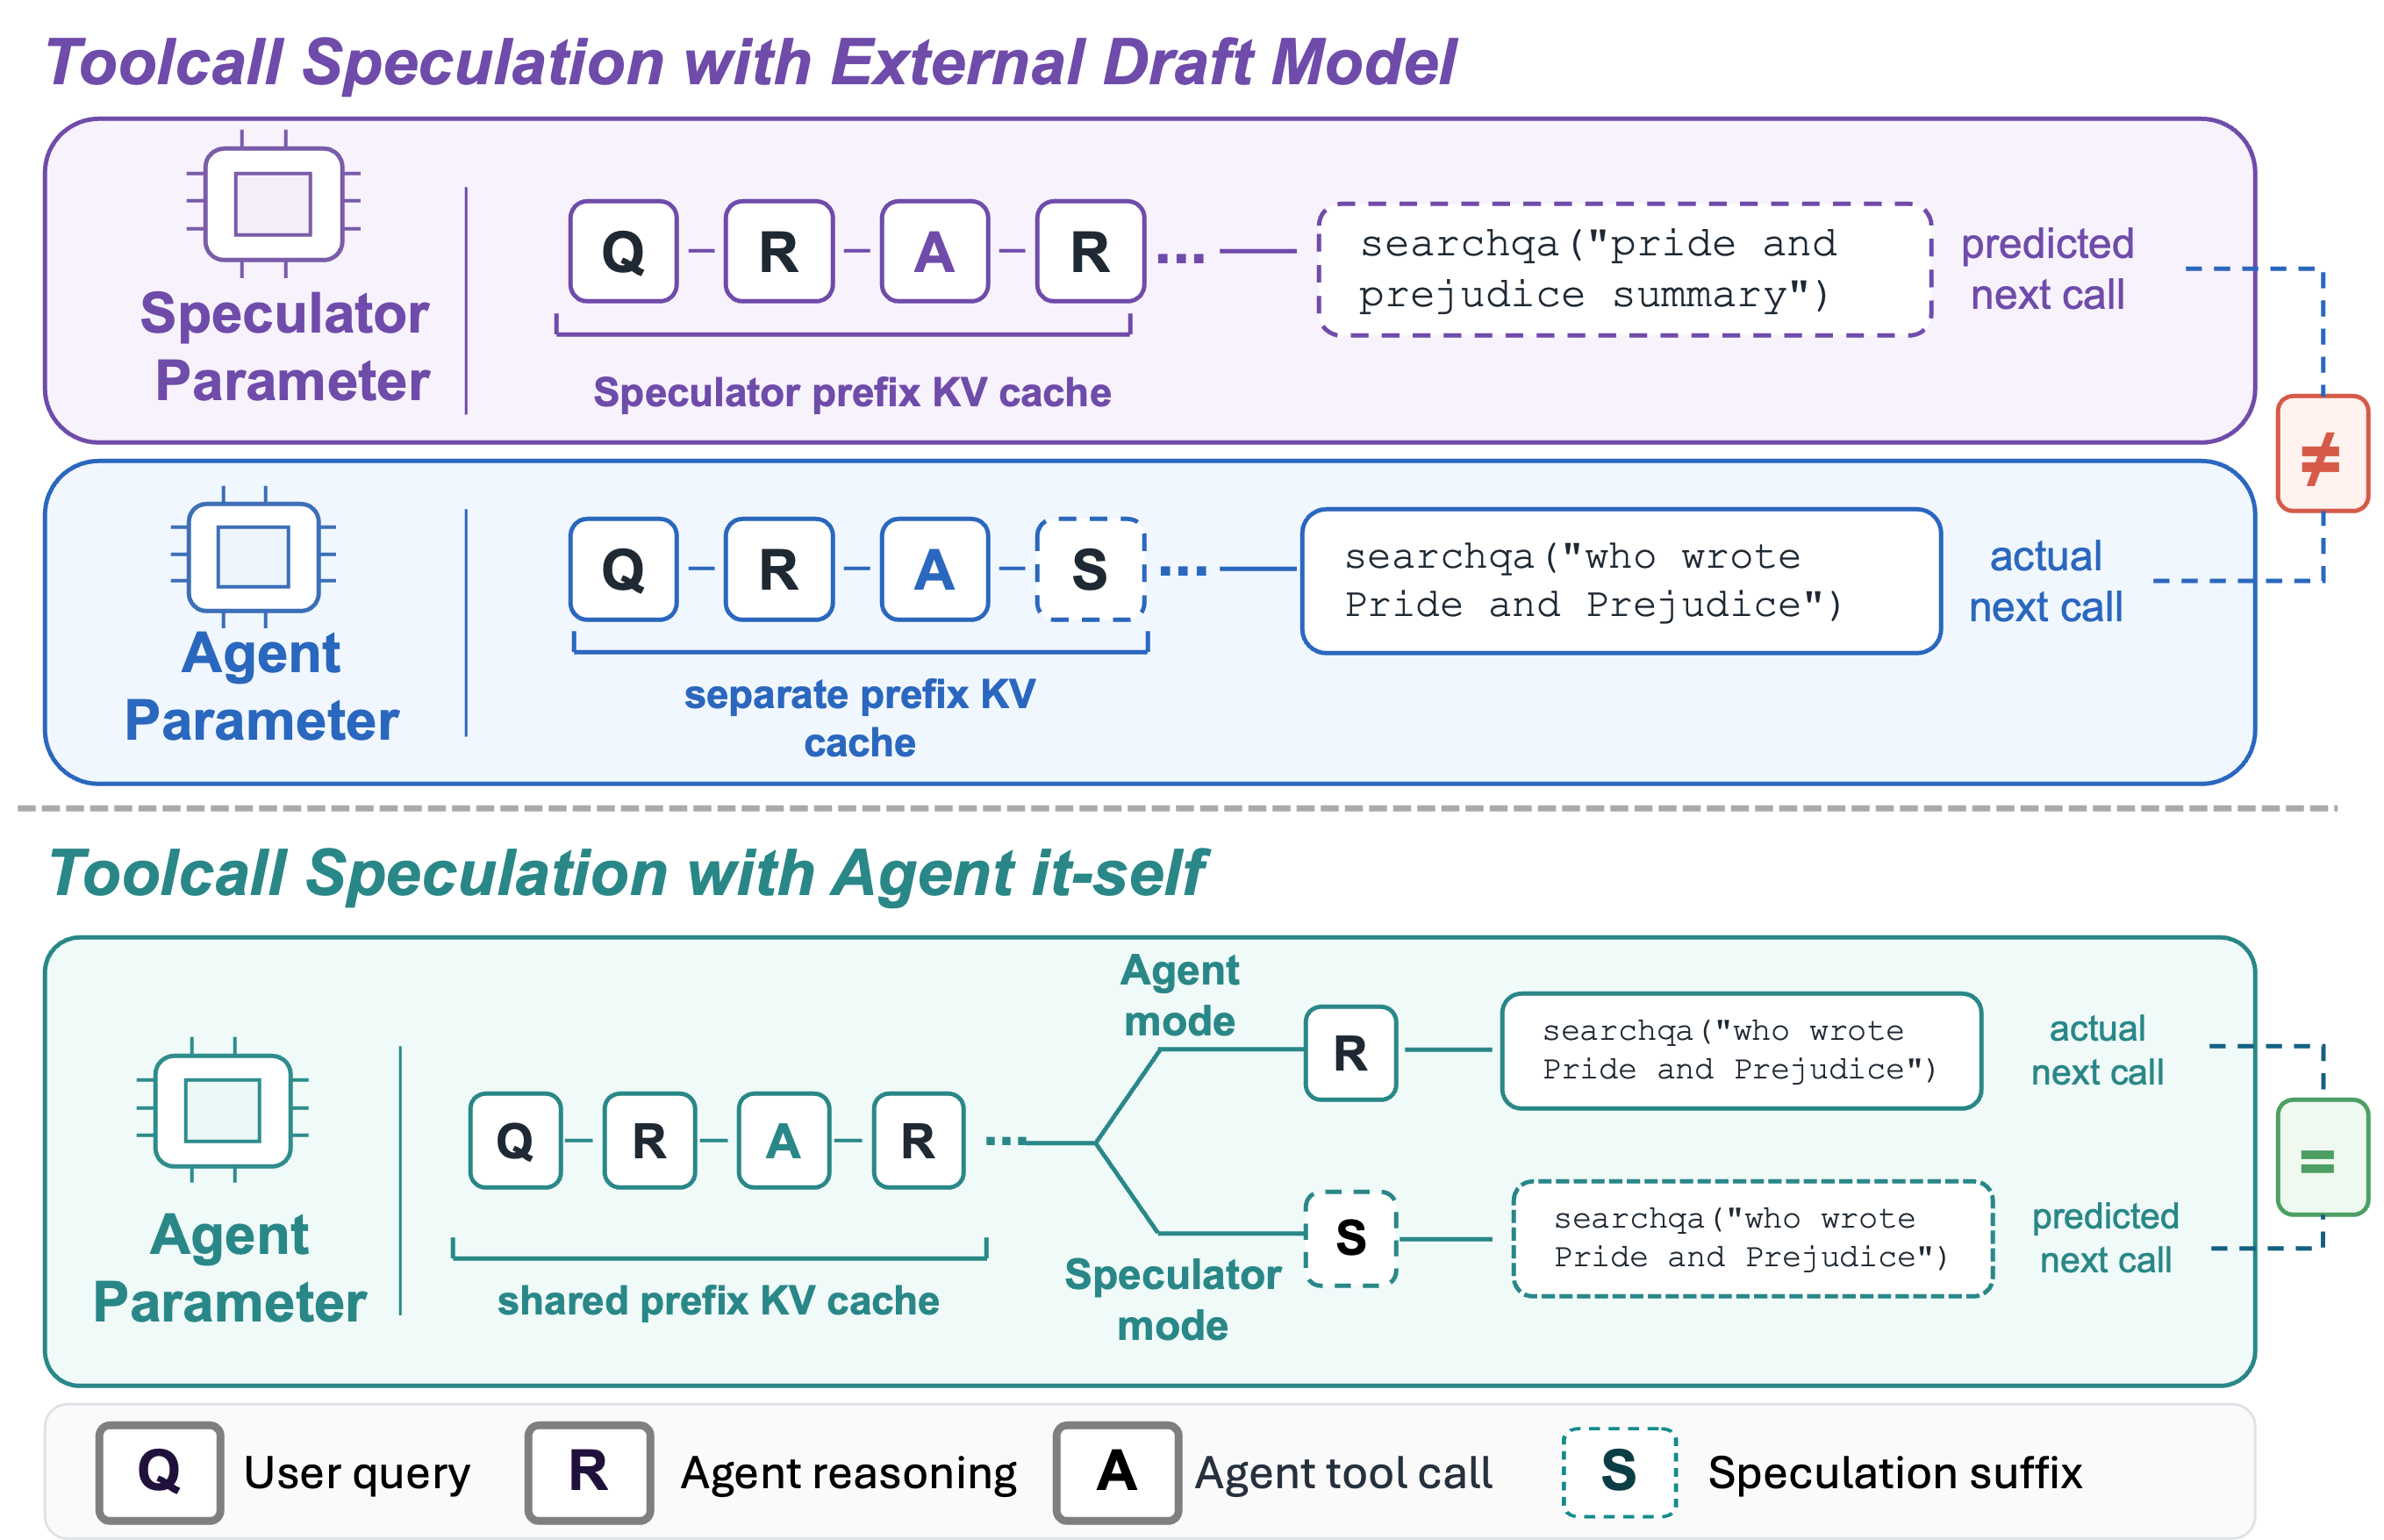
\includegraphics[width=0.95\linewidth]{intro_self_speculation.png}
    \vspace{1mm}
    \caption{External versus self tool-call speculation. The upper panel shows
    an external draft model with separate parameters and KV cache, which 
    predict a different next call due to the speculator--agent gap. The lower panel shows
    self-speculation with a shared prefix KV cache.}
    \label{fig:self-speculating-overview}
    \vspace*{-0.2in}
\end{figure}

Large language model (LLM) agents solve complex tasks by interleaving
natural-language reasoning with calls to external tools, including web search
engines, databases, code interpreters, and task-specific APIs~\citep{schick2023toolformer,patil2023gorilla,chen2023fireact,liu2024apigen}.
Recent work further trains and evaluates such agents in search, web,
function-calling, and long-horizon interaction settings~\citep{jin2025searchr1,song2025r1searcher,tan2025ragr1,qi2025webrl,qian2025toolrl,zhang2025toolr1,liu2026agentskills,luo2025agentlightning}.
These tools extend agents beyond their parametric knowledge by allowing them to
retrieve up-to-date information, execute computations, inspect structured
records, and interact with external environments. This flexibility, however,
comes at the cost of latency. Unlike token generation, tool calls often involve
remote services, network I/O, or even invoking another LLM as a sub-agent. As a result, agents may spend a substantial fraction of
their inference time waiting for tool results rather than performing token generation~\citep{nichols2025speculativetoolcalls,huang2025spagent,hooper2026speculativeinteraction},
making reduced waiting time central to responsive agents.

A promising approach is \emph{tool-call speculation}: issue likely future tool
calls before the agent explicitly produces them. A speculator observes an
intermediate trajectory, predicts the agent's next tool call, and executes that
call in parallel while the agent continues reasoning. If the prediction exactly
matches the agent's eventual tool call, the cached tool call result can be reused,
hiding the tool call latency. If it does not match, the
pre-executed result must be discarded. This exact-match reuse scenerio makes
tool-call speculation different from general tool use. Instead of predicting a general tool call, 
the speculator must produce the particular tool call that the deployed agent will actually take.

This requirement makes the design of the speculator especially important. Prior
work typically builds the speculator outside the deployed agent, either by using
a smaller LLM as an external draft model~\citep{ye2026speculativeactions,nichols2025speculativetoolcalls,huang2025spagent}
or by consulting cached tool call traces derived from
previous agent trajectories~\citep{zhong2026dualspec,sui2026paste}. These methods
show promising results to reduce latency, but they share a
fundamental limitation: the speculator is not the agent. An off-the-shelf draft
model approximates a generic tool-using assistant rather than the particular
agent being deployed. A cache-based method replays calls from previous
trajectories, which may correspond to different user queries, different
intermediate reasoning states, or outdated environments. In both cases, the
speculation methods remain separated from the actual deployed agent.

We refer to this separation as the \emph{speculator--agent gap}: conditioned on
the same intermediate agent trajectory, the speculator and the deployed agent may
choose different next tool calls. Figure~\ref{fig:self-speculating-overview}
illustrates this gap, where an external draft model maintains a separate set of model parameters and KV-cache
and predicts a different call than the target agent eventually issues. In
Section~\ref{sec:empirical-self-speculate}, we find that the gap appears even
within the same model family: smaller Qwen draft models often fail to match the
4B target agent's next tool call, while the 4B agent itself is already a stronger off-the-shelf speculator when prompted to predict
its own next call. 
External speculators also introduce practical systems overhead, including an additional
model weights, a separate KV cache, or historical traces.

These observations suggest a simpler speculator design: rather than aligning a separate
speculator to the agent, the agent itself can speculate. This leads to the
central research question: \emph{Can we train a agent to better
anticipate its own next tool call while preserving task solving performance?}

We therefore present a \emph{self-speculating agent}: a single model trained to
operate in two modes. In \emph{agent mode}, the model follows the standard
agentic trajectory, producing reasoning, tool calls, observations, and final
answers. In \emph{speculator mode}, the same model receives an intermediate
trajectory together with a short speculation suffix and directly predicts the
next structured tool call. Because both modes share the trajectory prefix,
inference can reuse the agent's prefix KV cache and branch only for the
speculation suffix and candidate call. Unlike external speculation, this
approach does not require serving an auxiliary draft model or maintaining a
historical tool-call traces.

However, training such an agent is nontrivial. Self-speculation couples two
objectives that are naturally imbalanced: the agent must remain effective at
solving tasks, while also becoming accurate at predicting its own next tool call
from partial trajectories. The two modes differ substantially in output
distribution, and naively training the agent to improve speculation can hurt
agent performance. To address this problem, we introduce \emph{joint agent-speculator RL}
During the RL process, we sample agent rollouts from the current policy, construct
speculator queries from those rollouts, and optimize each mode in an alternating procedure.
This keeps the speculator mode on-policy: it is trained on the same contexts that arise from the current agent, 
rather than on stale rollouts or data from a different model. We further stabilize this joint training with several training-time techniques, such as optimizer resets at mode switches.

Experiments across agentic search QA and conversational tool
use agentic tasks show that joint agent-speculator RL substantially improves speculation performance
while preserving task performance. For Qwen3-4B and Qwen3.5-4B, average 
next tool-call Hit@1 score improves from 44.1 to 61.2 and from 48.9 to 66.3, respectively,
while average downstream task success remains stable or slightly improves.

Our contributions are as follows:
\begin{itemize}
    \item We identify the speculator--agent gap in agentic tool-use tasks where off-the-shelf draft models often fail to match the agent's next structured call and add serving overhead.
    \item We introduce a self-speculating agent, where one LLM switches between task-solving and next-call prediction modes.
    \item We propose joint agent-speculator RL, which trains speculation from the current agent's own rollouts while preserving task success.
\end{itemize}
